% !TEX root = ../tex/1-1.tex
% DGMとは何か、学習の目標
\begin{frame}{DGM(深層生成モデル)}
\begin{block}{DGM(Deep Generative Models)}
高次元データに対する確率分布を学習し、データセットに類似したサンプルの生成が可能なモデル\\
\end{block}

\vspace{-1em}

\begin{columns}[T]
\begin{column}{0.48\textwidth}
\begin{exampleblock}{\small 目標1 Realistic Generation}
\small 実際のデータと区別できないような\textbf{新しいサンプルを生成}
\end{exampleblock}
\end{column}

\begin{column}{0.48\textwidth}
\begin{exampleblock}{\small 目標2 Controllable Generation}
\small 生成過程を解釈可能な形での制御を可能に
\end{exampleblock}
\end{column}
\end{columns}

\vspace{1em}

\small モデルが表す確率分布:\boldmath{$p_{\phi}$}  実際のデータが従う確率分布\footnote{data distribution, true distributionとも呼び、一般に$p_{data}$自体は未知である}:$p_{data}$\unboldmath\\

\begin{itemize}
\item 有限個のデータセットに対し\\
$p_{\phi}$と$p_{data}$間の損失関数を最小化→${\phi}$を最適化
\end{itemize}

\begin{exampleblock}{}
⇒つまり$p_{\phi}(x)\approx p_{data}(x)$が理想的\\
しかし$p_{data}(x)$が不明なので手元にある$p_{data}$から得られた\\サンプル$x^{(1)},x^{(2)},...x^{(N)}$から$\phi$を学習 ⇒ 分布を推定
\end{exampleblock}
\end{frame}
%=======================================================
\begin{frame}{1.1.1 Mathematical Setup -Goal of DGM}
\begin{exampleblock}{}
    前提：未知の分布$p_{data}$からサンプリングした有限個のサンプル\[
\left\{\mathbf{x}^{(i)}\right\}_{i=1}^{N}が手元にある
\]
\end{exampleblock}
\small $p_{data}$を表す式、新しいサンプルを生成する方法もわからない\\
⇒そこでパラメータ$\phi$を持つ深層ネットで\textbf{モデル分布}$p_{\phi}(x)$を構成\footnote{pは文脈により($p_{data}$)確率分布または($p_{data}(x)$)確率密度関数}
\begin{block}{DGMの目標}
    \centering$\phi^{*}$を学習して$p_{\phi^{*}}(\boldsymbol{x})\approx p_{data}(\boldsymbol{x})$\\
    $p_{\phi}$をGenerative model（生成モデル）という
\end{block}
⇒未知の$p_{data}$から得られた有限データを使って$p_{\phi^{*}}\approx p_{data}$となる\\
モデルを学習し、そこから新しいデータを生成する\\
\vspace{1em}
\textbf{生成}：学習済みの分布から新しいサンプルをサンプリングすること\\
\centering $\boldsymbol{x}\sim p_{\phi}$とすると$\boldsymbol{x}$は新しいサンプル

\end{frame}
%=======================================================
\begin{frame}{Figure 1.1：DGMの目標}
    \centering
    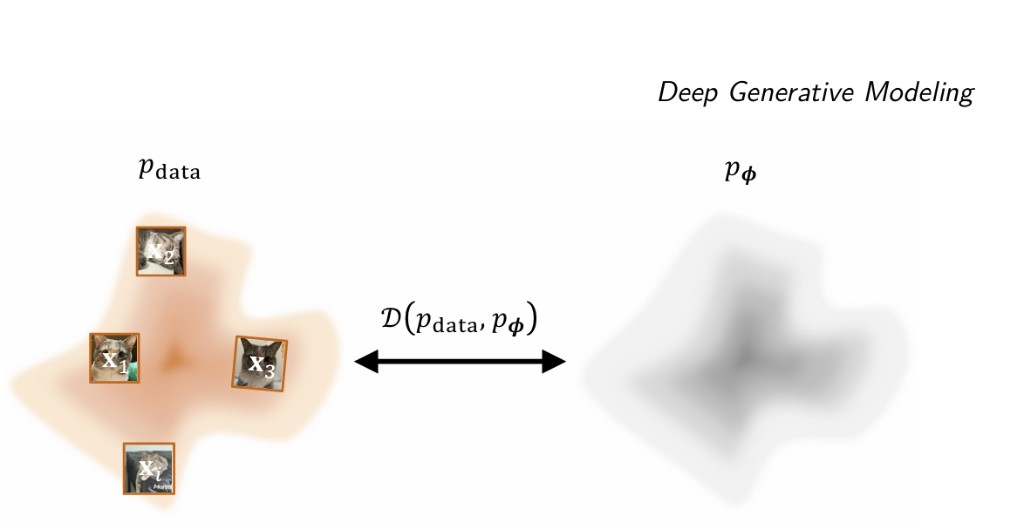
\includegraphics[
        width=\textwidth,
        height=0.55\textheight,
        keepaspectratio
    ]{figure1-1.png}
    \begin{exampleblock}{目的}
    モデル分布$p_{\phi}(x)$とデータ分布$p_{data}(x)$の隔たりを最小化\\
    \end{exampleblock}
    \small 未知の分布$p_{\mathrm{data}}(x)$から得た有限個の独立同分布（i.i.d.）サンプル$\{\boldsymbol{x}^{(i)}\}_{i=1}^{N}$を用いて$\phi$を学習し、新たなサンプルを生成する。

\end{frame}
